\PassOptionsToPackage{svgnames}{xcolor}
\documentclass[spanish, utf8,handout]{beamer} %
\usepackage[T1]{fontenc}
\usepackage{mathpazo}
\usepackage[spanish]{babel}
\usepackage{amsmath,mathrsfs,amsfonts,amsthm}
\usepackage{tikz}
%\usetheme[numbering=fullbar]{focus}%progressbar
%\definecolor{main}{RGB}{92, 138, 168}
%\definecolor{background}{RGB}{240, 247, 255}
\usepackage[
	audience=english
%	audience=spanish,
%	audience=german
]{beameraudience}

%\newcommand{\progressbar}{%
%	\pgfmathsetmacro{\theta}{360/\inserttotalframenumber*\insertframenumber}
%	\begin{tikzpicture}[scale=0.035]
%	\fill[yellow] (0,0) circle (9);
%	\fill[red] (0,0) -- (9,0) arc (0:-\theta:9);
%	\fill[white] (0,0) circle (5);
%	\node at (0,0) {\insertframenumber};
%	\end{tikzpicture}
%}

%\setbeamertemplate{footline}{\hfill \progressbar}

\usepackage{textpos}
\usepackage{mathtools}
\usepackage{dsfont}


%\useoutertheme{splitwithminiframes}
%\useoutertheme{sidebarwithminiframes}
%\usecolortheme[cautious]{owl}
\theoremstyle{definition}
\newtheorem{remark}{Observación}

\usetheme{CambridgeUS}
\usecolortheme{dolphin}
\useinnertheme{rectangles}
%\useoutertheme[hooks]{tree}

\usefonttheme[onlymath]{serif}

%\setbeamercovered{transparent}
\setbeamercovered{dynamic}

\setbeamertemplate{background canvas}{
\includegraphics[height=\paperheight]{background}}
\setbeamertemplate{footline}[frame number]{}
\setbeamertemplate{navigation symbols}{}
\setbeamertemplate{footline}{}
\setbeamertemplate{headline}{}
\setbeamertemplate{blocks}[rounded][shadow=false] 

\title[Teorema de los cuatro colores]{\Huge\sffamily Relaciones de recurrencias}
\subtitle{Ecuaciones en diferencias y análisis en escalas de tiempo}

\author[Grupo N$^\circ6$]{%
	\texorpdfstring{%
		\begin{columns}
			\column{.3\linewidth}
			\centering
			C. Aznarán Laos %\inst{1,2}
			\column{.3\linewidth}
			\centering
			F. Cruz Ordoñez %\inst{1,2}
		\end{columns}
		\vspace{12pt}
		\begin{columns}
			\column{.3\linewidth}
			\centering
			G. Quiroz Gómez %\inst{1,2}
			\column{.3\linewidth}
			\centering
			J. Micha Velasque %\inst{1,2}
		\end{columns}
		\vspace{12pt}
		\begin{columns}
			\column{.3\linewidth}
			\centering
			D. García Fernández %\inst{1,2}
%			\column{.3\linewidth}
			\centering
		\end{columns}
	}
	{Author 1, Author 2, Author 3}
}

\institute[FC -- UNI]{\large%\inst{1}
	Facultad de Ciencias \and%\inst{2}
	Universidad Nacional de Ingeniería
}
\date{21 de junio del 2019}

\graphicspath{{images/}}

\AtBeginSubsection[]
{
	\begin{frame}<beamer>
		\frametitle{\contentsname}
		\tableofcontents[
		currentsection,
		sectionstyle=show/show,
		subsectionstyle=show/shaded/hide%-show/shaded/hide
		]
	\end{frame}
}
\begin{document}

\frame{\titlepage}

%\begin{frame}[plain]
%	\maketitle
%\end{frame}
\begin{frame}{\contentsname}\transblindsvertical
	\tableofcontents
\end{frame}

\section{Introducción}

\subsection{Relación de recurrencia}
\subsubsection{Con coeficientes constantes}
\subsubsection{Homogénea}

\subsection{Ecuaciones en diferencias}
\begin{frame}
	\frametitle{Ecuaciones en diferencias(E.D)}
	\begin{block}{Definición 1:}
	Una ecuación en diferencias es una expresión de la forma:
	$$
	G(n,f(n),f(n+1),\ldots,f(n+k))=0, \; \forall n \in \mathbb{Z}
	$$
	\emph{Obs:}\hspace{2mm}$ f $ está definida en $ \mathbb{Z} .$
	\end{block}
	\begin{block}{Definición 2:}
	Se le llama orden de una E.D a la diferencia entre el operador diferencia mayor y menor que aparezcan en la ecuación; es decir, $ n+k-n=k $
	\end{block}
\begin{block}{Ejemplo}
	$ f(n+3)-f(n+1)-5f(n)=n $ es una E.D de orden $ 3 .$\\$ f(n+3)-f(n+1)=n^{2}-3 $ es una E.D de orden $ 2 .$
\end{block}
\end{frame}
\begin{frame}
\begin{block}{Definición 3:}
	Se le llama \emph{solución} de una E.D a toda sucesión $  \{f(0),f(1),\ldots,f(n),\ldots \} $ que la satisfaga,ahora se le llama \emph{solución general} de una E.D al conjunto de todas las soluciones que tendrán tanto parámetros como orden tenga la ecuación.La determinación de estos parámetros, a partir de unas
	condiciones iniciales, nos proporcionará las distintas soluciones particulares.
\end{block}
\begin{block}{Ejemplo 3.1:}
	$ f(n+1)-f(n)=3 $ es una E.D de orden uno cuya solución general es $ f(n)=3n+c $.Si consideramos unas condiciones iniciales,por ejemplo ,$ f(0)=2$, entonces $ f(0)=3\times0+c=c,$ por tanto $ c=2 $ y la solución particular es $ f_{p}(n)=3n+2.$Es decir, la solución es la sucesión $ f_{p}(n)=\{2,5,8,11,\ldots\} $
\end{block}
\end{frame}
\begin{frame}
	 \begin{block}{Ecuaciones en diferencias lineales(E.D.L)}
	 Llamamos ecuación en diferencias lineal de orden $ k $ a toda expresión de la forma:
	 $$
	 f(n+k)+a_{1}(n)f(n+k-1)+\ldots+a_{k-1}(n)f(n+1)+a_{k}(n)f(n)=b(n)
	 $$
	 \emph{Obsv:}\hspace{2mm}$ a_{k}(n)\neq0$
	 \end{block}
 \begin{block}{Clasificación:}
 	Las E.D.L se pueden clasificar en:\\
 	\begin{itemize}
 		\item Homogéneas si $ b(n)=0 .$
 		\item Completas si $ b(n)\neq0.$
 		\item De coeficientes constantes si $ a_{i}(n)=a_{i}, \forall i .$
 		\item De coeficientes no constantes si $ a_{i}(n)\neq a_{i} $ para algún $ i .$
 	\end{itemize}
 \end{block}
\end{frame}
\begin{frame}
	\begin{block}{Teorema 1:{\bf (Teorema de la existencia y la unicidad)}}
		Dada la ecuación:
		$$
		f(n+k)+a_{1}(n)f(n+k-1)+\ldots+a_{n-1}(n)f(n+1)+a_{n}(n)f(n)=0,
		$$
		y dados $ n $ números reales $ k_{0},k_{1},\ldots,k_{n-1} $ existe una única solución que verifica 
		$$
		f(0)=k_{0},f(1)=k_{1},\ldots,f(n-1)=k_{n-1}.
		$$
	\end{block}
\begin{block}{Teorema 2:}
	Toda combinación lineal de soluciones de una ecuación en diferencias lineal homogénea de orden $ n $ es también una solución.
\end{block}
\begin{block}{Corolario 1:}
	Las soluciones de una ecuación en diferencia lineal de orden $ n $ forman un espacio vectorial.
\end{block}
\begin{block}{Teorema 3:}
	La dimensión del espacio de soluciones de una ecuación en diferencias lineal de orden $ n $ es $ n .$
\end{block}
\end{frame}




%http://personal.us.es/pnadal/Informacion/leccion5ecdiferencias.pdf
\begin{frame}
	\begin{block}{Ecuaciones en diferencias de primer orden}
		
	\end{block}
	\begin{block}{Ecuaciones en diferencias de segundo orden}
		
	\end{block}
\end{frame}
\subsubsection{Número de Catalan}
\begin{frame}{Número de Catalan}
	\begin{block}{Triangulación}
		\begin{figure}
		\centering
		 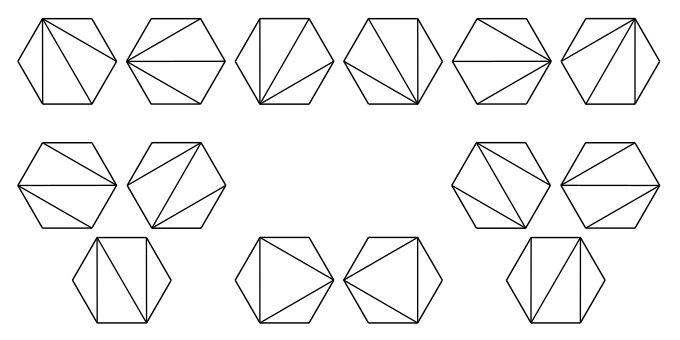
\includegraphics[scale=0.15]{ca1}
		\end{figure}
	\end{block}
\begin{block}{Caminos monótonos}
	\begin{figure}
		\centering
		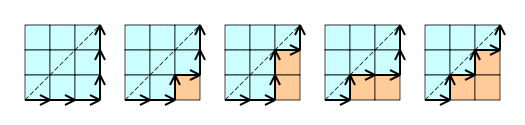
\includegraphics[scale=0.25]{ca2}
	\end{figure}
\end{block}
\end{frame}
\begin{frame}
	\frametitle{Aplicaciones}
\end{frame}
\subsubsection{Torre de Hanoi}
\subsubsection{Número de Ackermann}

\section{Realización numérica}

\subsection{Discretización}
\subsubsection{Método de Euler}
\subsubsection{Método de Runge-Kutta}

\section{Aplicaciones}

\subsection{Escalas de tiempo}
\subsubsection{Derivada fraccionaria}
\subsection{Módulo \texttt{timescale}}

\includeslide{}

\begin{frame}
	Hola
	\frametitle{Soluciones}
	%------------------------------------------------------------ 1
	\only<1>{
		\framesubtitle{The first frame subtitle}
		\begin{itemize}
			\item some text on slide 1
	\end{itemize}}
	%------------------------------------------------------------ 2
	\only<2>{
		\framesubtitle{The second frame subtitle}
		\begin{itemize}
			\item some text on slide 2
	\end{itemize}}
\end{frame}

\frame[t]{
	Una escala de tiempo es un conjunto cerrado $\mathds{T}$ bajo la topología estándar sobre $\mathds{R}$.

	Se define el operador salto posterior $\sigma\colon\mathds{t}\rightarrow\mathds{T}$ por \[ \sigma\left(T\right)\coloneqq\inf\left\{z\in\mathds{T}:z>t\right\} \]

	la granicidad $\mu\colon\mathds{T}\rightarrow\mathds{R}$ por \[ \mu\left(t\right)=\sigma\left(t\right)-t \] y función granicidad minimal $\mu_{\ast}\colon\mathds{T}\rightarrow\mathds{R}$ por \[ \mu_{\ast}\left(s\right)=\inf_{\tau\in\left[s,\infty\right)\cap\mathds{T}}\mu\left(t\right). \]

	Una función $f\colon\mathds{T}\rightarrow\mathds{C}$ es llamada $\Delta$--diferenciable si para cualquier $\varepsilon>0$ existe $\delta>0$ tal que para todo $s\in\left(t-\delta,t+\delta\right)\cap\mathds{T}$ y existe un número $f^{\Delta}\left(t\right)$ tal que \[ |\left[f\left(\sigma\left(s\right)\right)-f\left(s\right)\right]f^{\Delta}\left(s\right)\left[\sigma\left(t\right)-s\right]|\leq\varepsilon|\sigma\left(t\right)-s|. \]

	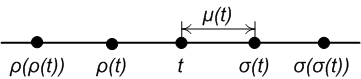
\includegraphics[width=0.4\paperwidth]{operators}
}

\frame{
	La integración se define de modo que $\int_{t}^{s}f^{\Delta}\left(\tau\right)\Delta\tau=f\left(t\right)-f\left(s\right)$.

	Si $\mathds{T}$ consiste únicamente de puntos aislados, entonces \[ f^{\Delta}\left(t\right)=\frac{f\left(\sigma\left(t\right)\right)-f\left(t\right)}{\mu\left(t\right)} \]

	y

\[
\int_{a}^{b}f\left(t\right)\Delta t=
\begin{cases}
	\sum_{t\in\left[a,b\right)\cap\mathds{T}}\mu\left(t\right)f\left(t\right),&\text{si }a<b.\\
	0, & \text{si } a = b.\\
	-\sum_{t\in\left[b,a\right)\cap\mathds{T}}\mu\left(t\right)f\left(t\right), & \text{si }a>b.
	\end{cases}
\]
}

\frame{
	Content...
}

\frame{text}

\frame{text} \frame{text} \frame{text} 

\appendix  
\frame[noframenumbering,plain]{text} 

\setbeamertemplate{footline}
{%
	\hbox{%
		\begin{beamercolorbox}[wd=.3\paperwidth,ht=7.8pt,dp=3pt,center]{author in head/foot}\insertshortauthor
		\end{beamercolorbox}%
		\begin{beamercolorbox}[wd=.4\paperwidth,ht=7.8pt,dp=3pt,center]{title in head/foot}\insertshorttitle
		\end{beamercolorbox}%
		\begin{beamercolorbox}[wd=.3\paperwidth,ht=7.8pt,dp=3pt,center]{date in    head/foot}\insertshortdate\hspace*{5mm}%	
		\end{beamercolorbox}  
	}% 
} 

\addtobeamertemplate{footline}{}{%
	\begin{textblock*}{100mm}(0.94\textwidth,-7mm)
		\progressbar
	\end{textblock*}
}


%\begin{frame}{Title}
% all version
%\end{frame}

%\justfor{english}{
%    \begin{frame}
%    English Slide
%    \pause
%    tba
%    \end{frame}
%}
%
%\justfor{spanish}{
%    \begin{frame}
%    Spanish Slide
%    \pause
%    tba
%    \end{frame}
%}
%
%\justfor{german}{
%    \begin{frame}
%    Deutcher Text
%    \pause
%    wird noch angekündigt
%    \end{frame}
%}

\end{document}
https://www.i-ciencias.com/pregunta/35252/termino-comun-para-las-ecuaciones-diferenciales-y-de-relaciones-de-recurrencia

@book{book:{2135209},
	title =     {Intelligent computations : abstract fractional calculus, inequalities, approximations},
	author =    {Anastassiou, George A},
	publisher = {Springer},
	isbn =      { 978-3-319-66936-6,3319669362,978-3-319-66935-9 },
	year =      {2018},
	series =    {Studies in computational intelligence 734},
	edition =   {},
	volume =    {},
	url =       {http://gen.lib.rus.ec/book/index.php?md5=edcebea5cf073b0368a47fba1cb9b635}}


Dada la ecuación en diferencias lineal
de coeficientes constantes y de orden $ k $ :
$a_{0}f(n + k) + a_{1}f(n + k ¡ 1) + \ldots + a_{k}f(n) = g(n)$,
el problema de hallar una función $ f $ definida en $ \mathbb{Z} $;
que verifique la ecuación, y tal que en los $ k $ enteros
consecutivos $n_{0}, n_{0}+1,\ldots ,n_{0}+k-1$ tome los valores
dados $c_{0}, c_{1},\ldots , c_{k-1}$; tiene solución única.
